
\newcommand{\p}{\textbf{p}}

\chapter{Nonparametric Models}

In this chapter we describe several closely related Bayesian nonparametric models for inducing categories in a synchronous context-free grammar.  Our nonparametric models are variations on Latent Dirichlet Allocation (LDA) model of \cite{blei:2003}.  Rather than modeling sentences (or sentence pairs), we assume that rule extraction heuristics determine the set of valid constituents and grammar rules, and so our task is only to determine the category labels.  As discussed in the previous chapter, we make the critical assumption that each phrase (or pair), $\p$, can be clustered on the basis of the contexts it occurs in.  We therefore define a generative model of a corpus that consists of collections of contexts (one context collection for each phrase pair type).

\section{Model}

The high-level structure of our model is as follows: each observed phrase (pair), $\p$, consists of a finite mixture of categories, $\theta_{\p}$.  The list of contexts $C_{\p}$ is generated as follows.  A category type $z_i$ is drawn from $\theta_{\p}$, and this generates the observed context, $\textbf{c}_i$, according to a category-specific distribution over contexts types, $\phi_{z_i}$.  Since we do not know the values of $\theta_{\p}$ and $\phi_z$, we place priors on the distributions, to reflect our prior beliefs about the shape these distributions should have and infer their values from the data we can observe.  Specifically, our {\emph a priori} expectation is that both parameters will be relatively peaked, since each phrase, $\p$, should relatively unambiguous belong to particular category, and each category to generate a relatively small number of context strings, $\textbf{c}$.

To encode these prior beliefs, we make use of Pitman-Yor processes \citep{pitman:1997}, which can capture these intuitions and which have already been demonstrated to be particularly effective models for language \citep{teh:2006,goldwater:2006}.

Our models assume a fixed number of categories, $K$. The category type, $z \in \{ 1 , 2 , \ldots , K \}$, is generated from a PYP with a uniform base distribution:
\begin{align*}
z &| \p & \sim \theta_{\p} \\
\theta_p &| a_{\p},b_{\p},K & \sim \textrm{PYP}(a_{\p},b_{\p},\textrm{Uniform}(K))
\end{align*}
\noindent Alternatively, we used hierarchical PYP process which shares statistics about the use of categories across phrases:
\begin{align*}
z &| \p & \sim \theta_{\p} \\
\theta_{\p} &| a_{\p},b_{\p} & \sim \textrm{PYP}(a_{\p},b_{\p},\theta_0) \\
\theta_0 &| a_0,b_0,K & \sim \textrm{PYP}(a_0,b_0,\textrm{Uniform}(K))
\end{align*}

\noindent Each category $z$ token then generates the context $\textbf{c}_i$. We again model this using a PYP, which will tend to cluster commonly used contexts across phrases into a single category. Additionally, by using hierarchical PYPs, we can smooth highly specific contexts by backing off to less specific contexts (e.g., composed of fewer words or word classes).

The most basic version of our model uses a uniform prior base distribution over contexts:

\begin{align*}
\textbf{c} |& z & \sim \phi_z \\
\phi_z |& a_z,b_z & \sim \textrm{PYP}(a_z,b_z,\textrm{Uniform}(|V|^2))
\end{align*}

\noindent TODO. For contexts with more than a single word on either side, we typically backed off from a 

\begin{align*}
\textbf{c} |& z & \sim \phi_z \\
\phi_z |& a_z,b_z, \phi_0 & \sim \textrm{PYP}(a_z,b_z,\phi_0(\cdot|z) \times \textrm{Uniform}(|V|^2)) \\
\phi_0 |& a_0,b_0 & \sim \textrm{PYP}(a_z,b_z,\phi_0(\cdot|z))
\end{align*}

\noindent Figure~\ref{fig:np_plate} shows a plate diagram for the model.

\begin{figure}
\begin{center}
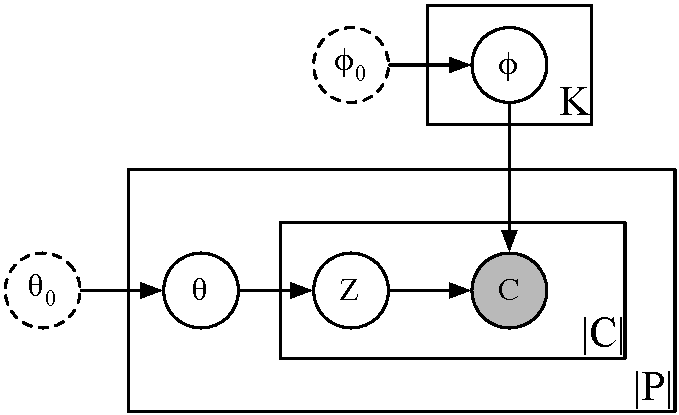
\includegraphics[scale=0.75]{pyp_clustering/np_plate.pdf}
\vspace{-0.3cm}
\end{center}
\caption{Plate diagram for the nonparametric clustering model (hyperparameters omitted).  Dashed circles indicate variables that may not be present in every model.}
\label{fig:np_plate}
\end{figure}

\subsection{Inference}

Inference in this model was performed using Gibbs sampling \citep{geman:1984}, with the continuous parameters ($\theta_{\p}$, $\phi_z$, etc.) integrated out.  For the experiments reported below, we sampled for 1000 iterations, initializing by assigning every context in a phrase entirely to a random category.  New values for the PYP hyperparameters were resampled using slice sampling every 10 samples \citep{neal:2000,johnson:2009}. The final sample was used to estimate $p(z|\textbf{c},\p)$, and each phrase occurrence was labelled with the $z$ that maximized this probability (TODO check this).

\section{Experiments}

\subsection{Number of categories}

\subsection{Context types}


